%# -*- coding: utf-8-unix -*-
%%==================================================
%% chapter02.tex for SJTU Master Thesis
%%==================================================

\chapter{实验分析}
\label{chap:evaluation}

本章节将通过综合性的负载和评测软件来测试SCache对Spark性能的优化效果。
首先我们运行了一个只包含一个shuffle的简单DAG工作来分析硬件利用率的变化。
同时也从改工作中具体每个任务的角度来分析SCache的优化带来的影响。
之后我们使用了一个公认的含有大量shuffle数据的测试程序Terasort\cite{terasort}来测试不同分区函数下SCache带来的优化。

为了证明SCache能在真实生产环境中带来性能的提升,我们也通过Spark TPC-DS\footnote{https://github.com/databricks/spark-sql-perf}的测试程序来对SCache的优化效果进行测试。

最后我们测试了有权重的水塘采样过程给Spark计算带来的开销。

简短来讲,在SCache的帮助下,可以减少Spark计算过程中89\%的shuffle时间开销。
同时,在单shuffle的DAG程序中,SCache可以帮助Spark实现在reduce阶段75\%的性能提升。
对于Terasort的reduce阶段,在SCache的帮助下可以实现50\%的性能提升。
并且通过启发式预调度算法,相较于Spark调度所产生的经过网络的shuffle数据体积,SCache的优化在加快reduce阶段执行的同时并不会引入额外的网络负载。
在标准的分布式数据库查询评测程序TPC-DS的测试中,经过SCache对shuffle的优化,可以为其中的查询提供接近40\%的平均查询时间优化,效果十分显著。

\section{实验平台搭建}

我们在目前应用广泛的Spark分布式计算框架1.6.2版本中实现了SCache的守护进程,并且通过修改Spark任务调度器(DAGScheduler和TaskSchedulerImpl)来实现了对DAG中shuffle信息和相关任务信息的提交,SCache附属调度器调度结果的获取和采样程序的插入等。
同时,我们租用了亚马逊AWS EC2中50个m4.xlarge类型的节点作为测试平台,并且部署修改后的Spark和SCache。
每个节点的配置如下表所示:
\begin{table}[!hpb]
    \centering
    \bicaption[tab:ec2]{测试平台节点配置}{测试节点平台配置}{Table}{Configuration of Testbed Instance}
    \begin{tabular}{ | m{5cm} | m{8cm} | }
        \hline
        \multicolumn{2}{| c |}{Configuration of Testbed Instance}\\ [0.5ex]
        \hline
        \hline
        Instance Type & m4.xlarge \\ \hline
        CPU & 2.3 GHz Intel Xeon E5-2686 v4 (Broadwell) / 2.4 GHz Intel Xeon E5-2676 v3 (Haswell) \\ \hline
        vCPU & 4 \\ \hline
        Memory & 16GB \\ \hline
        Storage & 8GB SSD, bandwidth 750 Mbps \\ \hline
        Network Bandwidth & N/A, ($\sim$300Mbps as we tested) \\ \hline
        OS & Ubuntu 14.04 LTS \\ \hline
        \hline
    \end{tabular}
\end{table}

其中每个计算节点为一个EC2的虚拟实例,包含了4个vCPU以及16GB的内存和8GB的SSD存储。
以上这些硬件性能保证了在测试过程中计算和内存不会限制测试程序的计算运行速度,同时也为shuffle数据的缓存提供了较充足的内存空间。
为了为Spark计算提供存储资源,我们还在集群上部署了Hadoop 2.7\cite{hadoop}来提供HDFS的分布式文件系统支持。
除此之外,我们在集群上的每个节点部署了采集CPU磁盘网络等硬件资源利用情况的程序。

\section{单shuffle依赖的DAG执行分析}

我们首先展示了运行与图\ref{fig:util}中一样的,只包含一个shuffle依赖的Spark程序,即Spark GroupByTest\cite{sparksource}。
在此次评测中,我们分别采用了不同体积的输入数据,同时为每一个计算阶段分配了5轮的任务。

在图\ref{fig:scache_util}中展示了在SCache优化下执行该单shuffle依赖的程序时的硬件资源使用情况。
需要注意的时在SCache的优化下,使得整个工作的执行时间缩短了50\%,因此图\ref{fig:scache_util}中横坐标代表的时间长度只有图\ref{fig:util}的一半。
首先可以看到的就是在图\ref{fig:scache_util}中出现了CPU资源利用率峰值和磁盘,网络这些硬件资源利用率峰值的重合。
这个表明了通过SCache对shuffle的解耦以及预取,使得节点中硬件资源的利用率和复用率得到了很大的提升。
在更细粒度的硬件资源管理下,SCache避免了在原先Spark中因为I/O的操作而无效的占用计算资源的情况。
同时,由于CPU的资源能被更即使的释放和更少的空置,是的整个集群在计算过程中始终保持较高的CPU利用率。
以上这些硬件资源利用率上的增加和复用率的增加从资源管理效率的角度证明了在SCache的帮助下,Spark的任务能够被更高效的执行,从而获得更好的性能。

\begin{figure}[!htp]
	\centering
	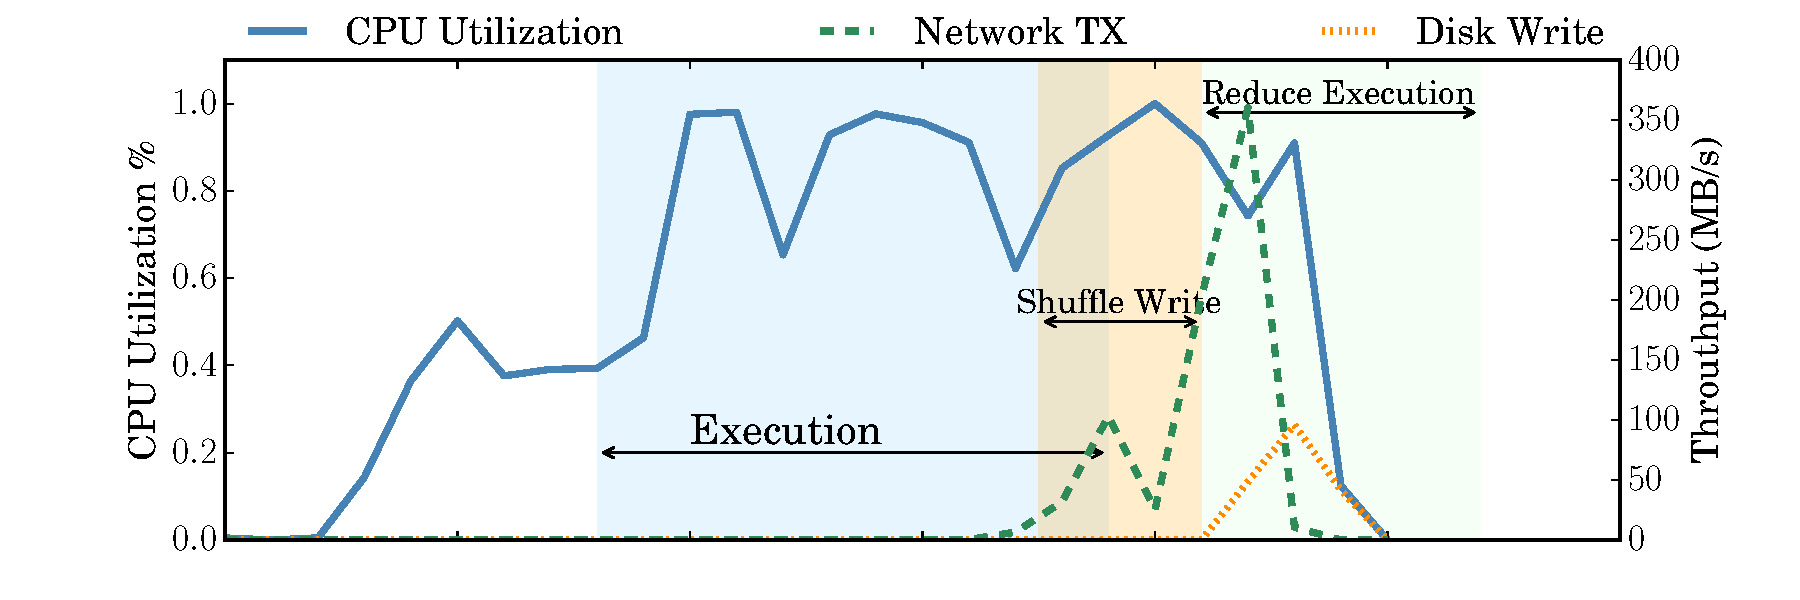
\includegraphics[width=\textwidth]{../../PPoPP-2018/fig/scache_util.pdf}
	\bicaption[fig:scache_util]{SCache优化后运行包含一个shuffle的Spark应用时的硬件资源利用率}{SCache优化后运行包含一个shuffle的Spark应用时的硬件资源利用率}{Fig}{CPU utilization and I/O throughput of a node
	during a Spark Single Shuffle Application With SCache}
\end{figure}

于此同时,我们也在计算任务层面对两者进行了比较。
如图\ref{fig:groupbymapstage}所示,可以看到在map阶段,随着输入数据的体积增加,SCache通过解耦合的方式提前释放CPU资源,同时通过内存拷贝的方式省略磁盘操作能给map阶段的性能带来一个较为显著的提升。
SCache的优化在map阶段平均可以带来约10\%的性能提升。
而图\ref{fig:groupbyreducestage}展示了shuffle数据预取对于需要大量shuffle数据传输的应用,能在reduce阶段带来非常显著的性能提升。
这些提升正是因为SCache通过在map阶段对reduce任务实行预调度和shuffle数据的预取,提前了原先Spark模式中shuffle开始的时间,有效的将网络传输时间隐藏在map计算阶段,从而减少了reduce计算阶段启动之后显示的shuffle等待时间,加快了reduce阶段的任务执行。
对于reduce阶段,SCache带来的性能提升较为显著,平均可以达到大约75\%。
两者相结合,在对单shuffle依赖的工作的优化过程中,SCache可以减少大约89\%的平均shuffle时间开销。

\begin{figure}[!htp]
    \centering
    \begin{minipage}[t]{0.47\textwidth}
	    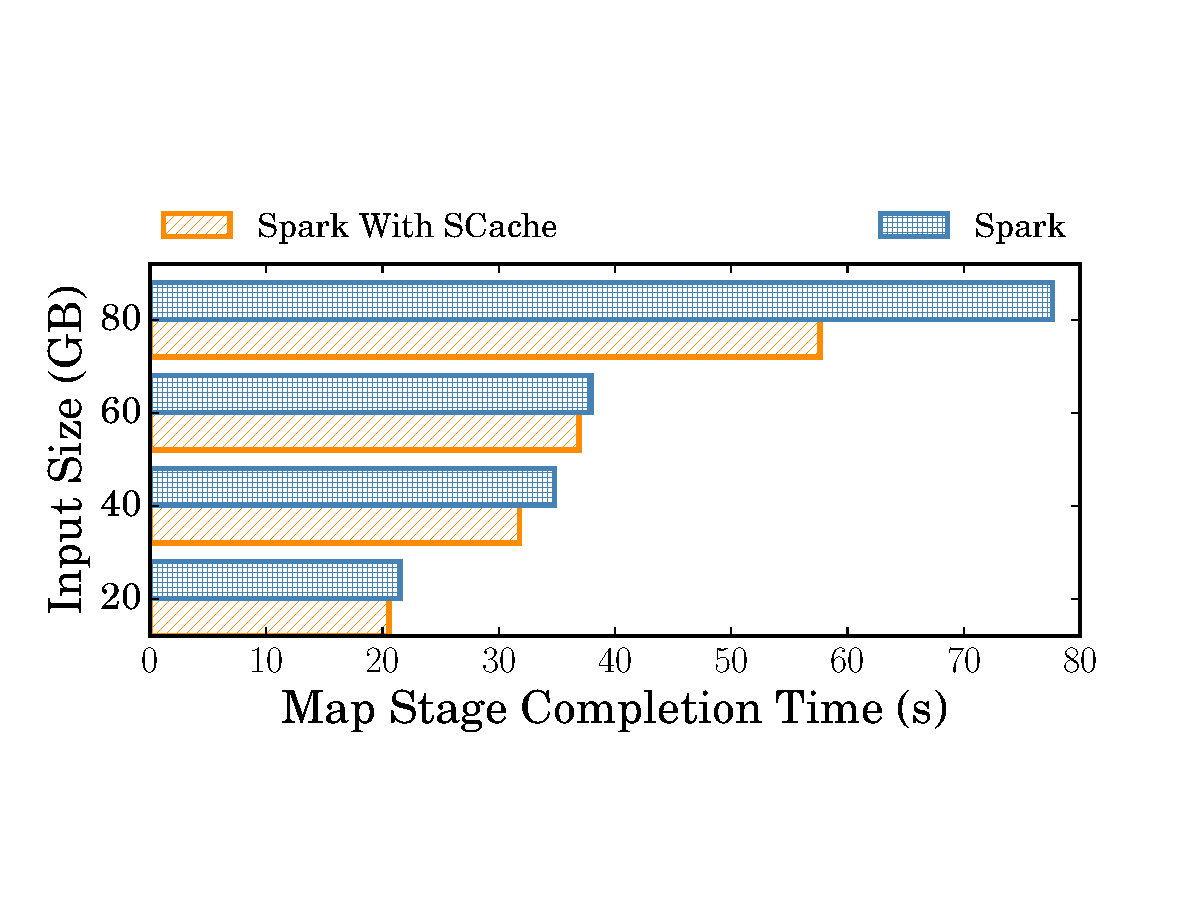
\includegraphics[width=\textwidth]{../../PPoPP-2018/fig/groupbymapstage.pdf}
	    \bicaption[fig:groupbymapstage]{单shuffle依赖工作的map阶段完成时间比较}{单shuffle依赖工作的map阶段完成时间比较}{Fig}{Map Stage Completion Time of Single Shuffle Test}
    \end{minipage}
    \begin{minipage}[t]{0.47\textwidth}
	    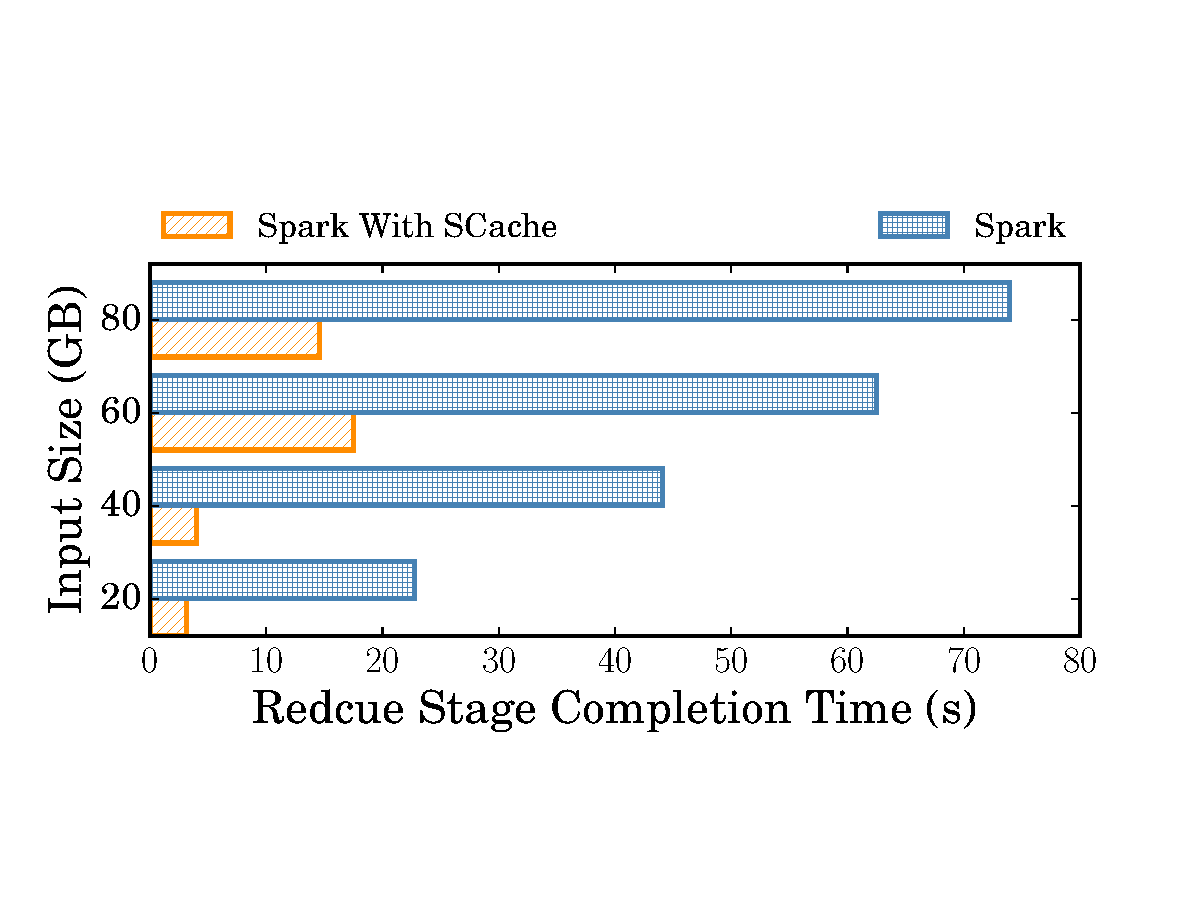
\includegraphics[width=\textwidth]{../../PPoPP-2018/fig/groupbyreducestage.pdf}
	    \bicaption[fig:groupbyreducestage]{单shuffle依赖工作的reduce阶段完成时间比较}{单shuffle依赖工作的reduce阶段完成时间比较}{Fig}{Map Stage Completion Time of Single Shuffle Test}
    \end{minipage}
\end{figure}

\begin{figure}[!htp]
    \centering
    \begin{minipage}[t]{0.47\textwidth}
	    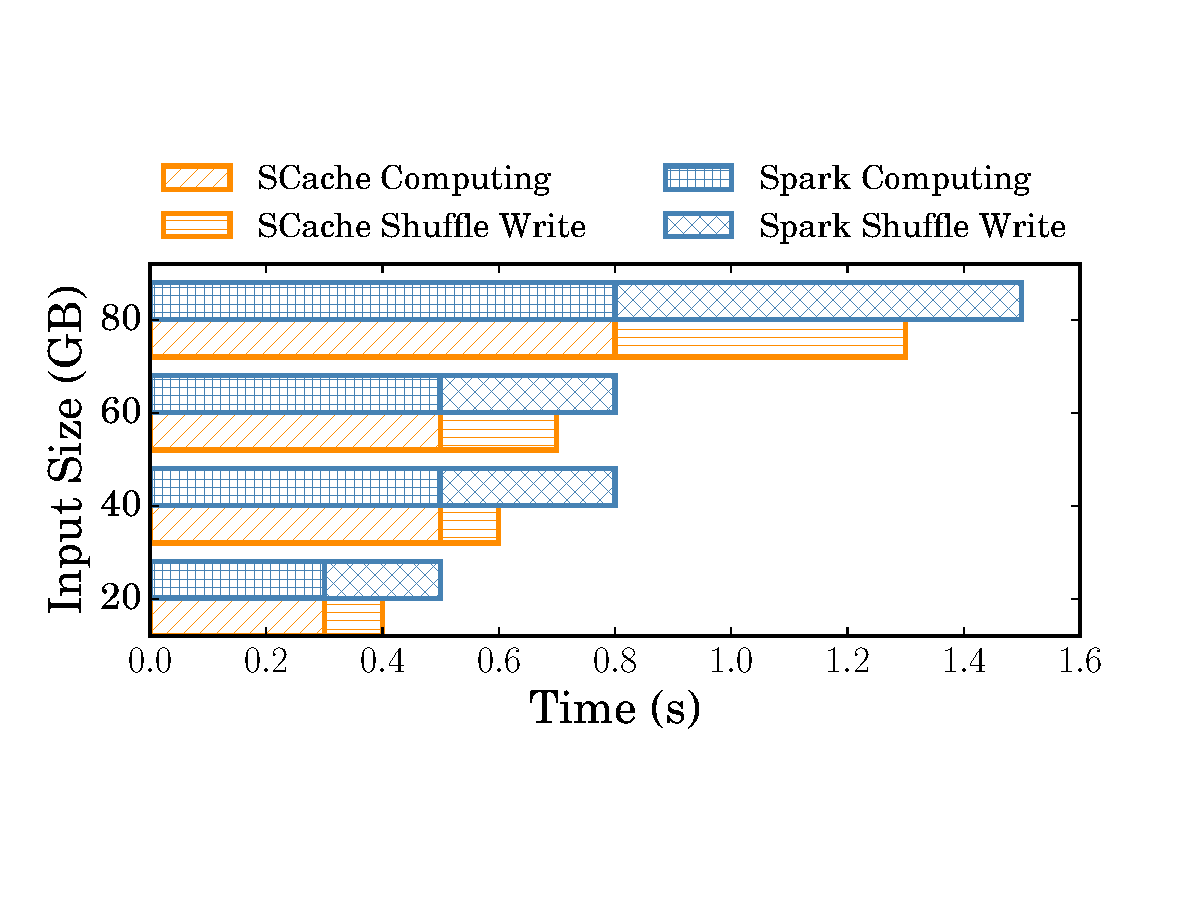
\includegraphics[width=\textwidth]{../../PPoPP-2018/fig/groupbymaptask.pdf}
	    \bicaption[fig:groupbymaptask]{单shuffle依赖工作的map阶段中位任务比较}{单shuffle依赖工作的map阶段中位任务比较}{Fig}{Median Map Task Completion Time of Single Shuffle Test}
    \end{minipage}
    \begin{minipage}[t]{0.47\textwidth}
	    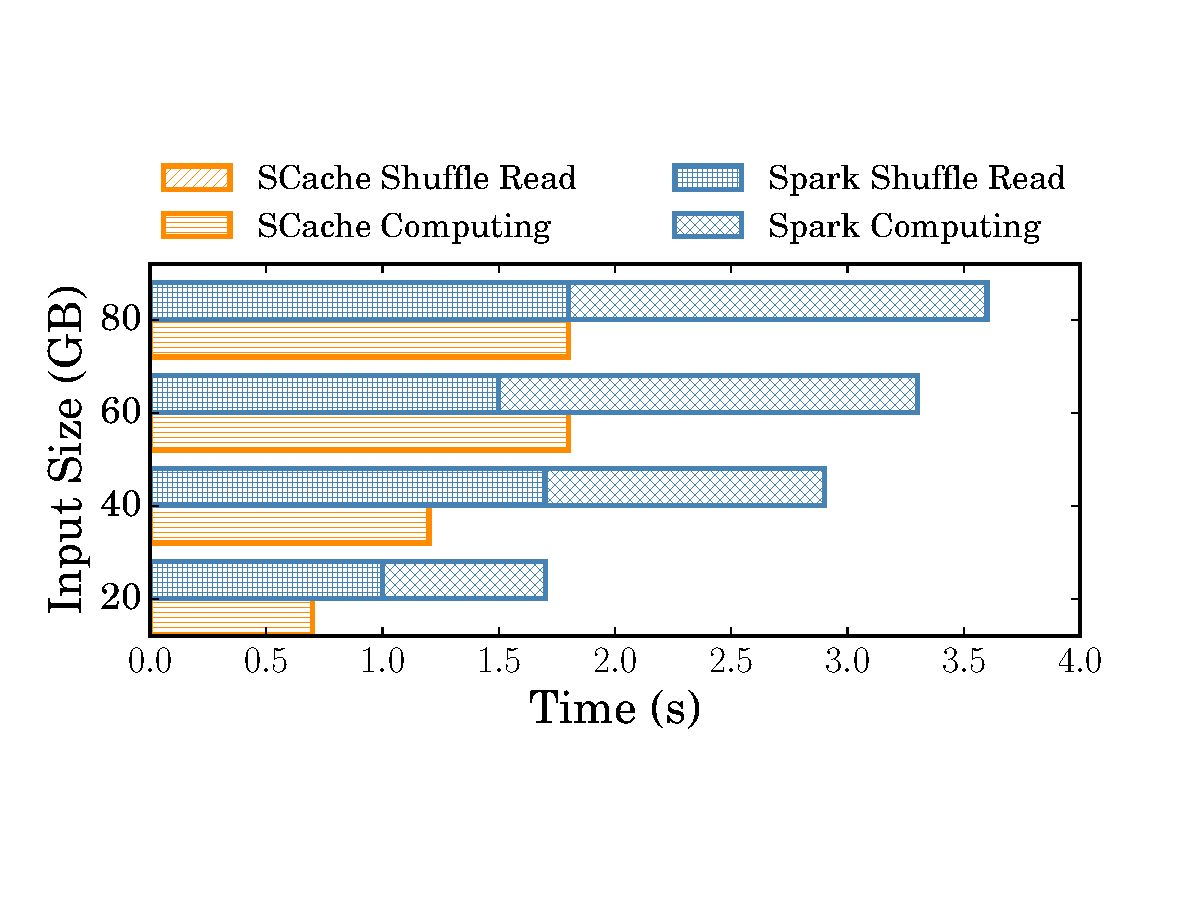
\includegraphics[width=\textwidth]{../../PPoPP-2018/fig/groupbyreducetask.pdf}
	    \bicaption[fig:groupbyreducetask]{单shuffle依赖工作的reduce阶段中位任务比较}{单shuffle依赖工作的reduce阶段中位任务比较}{Fig}{Median Reduce Task Completion Time of Single Shuffle Test}
    \end{minipage}
\end{figure}

具体到单个计算任务的角度,我们也记录了每个计算阶段中计算任务完成时间处于该阶段所有任务完成时间中位数的那个任务执行过程中具体的时间开销。
如图\ref{fig:groupbymaptask}和图\ref{fig:groupbyreducetask}所示,从任务执行过程中在各个部分的开销,能够进一步验证SCache优化过程的有效性。
在图\ref{fig:groupbymaptask}中的map阶段计算任务的执行过程比较中,可以看到通过SCache的将shuffle的磁盘写操作从map计算任务中解耦合之后,通过内存拷贝的方式可以优化大约40\%的shuffle数据写操作的开销。
之所以SCache的内存拷贝没有完全消除map计算任务中的shuffle写开销是因为在内存拷贝时,首先需要从Spark执行器的Java虚拟机中将shuffle数据移出。
而shuffle数据在Java虚拟机内存内部则是以Java类对象保存的,因此在将其移出内存空间时需要使用序列化的方法将类对象转换成字节码数组。
此处序列化的过程仍然会占用CPU的计算资源和时间\cite{makingsense},并且是不可避免的,因此在图\ref{fig:groubymaptask}中仍然能观测到shuffle写过程的时间开销。
所以通过对于任务的细粒度分析,也应证了图\ref{fig:groupbymapstage}中,在map阶段SCache解耦shuffle写的过程并没有带来如reduce阶段那么多的收益。

结合图\ref{fig:groupbyreducetask},可以观察到在Spark中,相较于map阶段shuffle写的时间开销,reduce阶段计算任务中shuffle读的开销占到整个任务执行时间的比例更大。
根据我们的实验检测发先该工作的reduce任务中,shuffle读取过程占到了reduce阶段计算任务的约50\%。
而这其中的大部分延迟是由网络传输带来的。
SCache通过在map计算阶段的早期对shuffle数据进行了预取,因此当reduce计算被Spark调度并且开始执行之前,通常情况下只有map计算阶段最后一轮的最后完成的几个任务产生的shuffle数据。
而这部分传输时间由于reduce任务调度的开销以及任务代码序列化等开销,也能被很好的隐藏起来。
一次在第一轮的reduce任务启动之后,SCache根据任务的预调度信息中的reduce任务ID等信息,已经将数据缓存在了内存当中。
因此可以看到在图\ref{groupbyreducetask}中,SCache可以通过shuffle数据预取将reduce计算任务开始之前的shuffle读等待时间几乎完全的隐藏起来。
也就说在SCache结合上下文的任务预调度与shuffle数据预取机制下,网络传输时间被很好的重叠在了map计算阶段和reduce计算阶段启动时期。






